\documentclass{article}
\usepackage[utf8]{inputenc}
\usepackage{listings}


\documentclass{article}
\usepackage[utf8]{inputenc}
\usepackage{listings}
\usepackage{xcolor}
\usepackage{graphicx}
\graphicspath{ {images/} }

%New colors defined below
\definecolor{codegreen}{rgb}{0,0.6,0}
\definecolor{codegray}{rgb}{0.5,0.5,0.5}
\definecolor{codepurple}{rgb}{0.58,0,0.82}
\definecolor{backcolour}{rgb}{0.95,0.95,0.92}

%Code listing style named "mystyle"
\lstdefinestyle{mystyle}{
  backgroundcolor=\color{backcolour},   commentstyle=\color{codegreen},
  keywordstyle=\color{magenta},
  numberstyle=\tiny\color{codegray},
  stringstyle=\color{codepurple},
  basicstyle=\ttfamily\footnotesize,
  breakatwhitespace=false,         
  breaklines=true,                 
  captionpos=b,                    
  keepspaces=true,                 
  numbers=left,                    
  numbersep=5pt,                  
  showspaces=false,                
  showstringspaces=false,
  showtabs=false,                  
  tabsize=2
}

%"mystyle" code listing set
\lstset{style=mystyle}


%"mystyle" code listing set
\lstset{style=mystyle}

\title{BTH004 - Laboratory assignment 1---\\
Multiple knapsacks problem and solutions}
\author{name: Zhao Shui--\\student ID: 201806150329}
\date{November 2020}

\begin{document}

\maketitle

\part{}
\section{Greedy algorithm}
\subsection{mainly description for the algorithm}
allocate knapsack for every items in the order of values per weight unit.
\subsection{implementation step}
\paragraph{step 1:} Create a new list calculate all items’ unit value(value per weight unit)in the items list and record its id, and then sort it in the order of unit value.
\paragraph{step 2:} For every item in the sorted list, allocate knapsack for the item in the order. if there are enough room in this knapsack , then include it in the current knapsack. If all knapsacks don’t have enough room for the item, then it will not be included in all knapsacks.
\paragraph{step 3:} All items have been allocated knapsack once, algorithm them end.
\subsection{two fit method are alternative: first fit and best fit}
\paragraph{first fit:}Once the current knapsack has enough room, then include in the knapsack immediately.
\paragraph{best fit:}Search all knapsacks, and look for the best knapsack(which left capacity most closed to the item weight)
\subsection{descriptions for some criteria}
\paragraph{termination criteria:}All items have been allocated knapsacks once, then end the algorithm.
\subsection{pseudo code}
\lstinputlisting[language=python]{pseudoCode1}
\subsection{code \& comment}
\lstinputlisting[language=python]{code1.m}
\subsection{correctness check \& test}
As you see in the code above, a lot of print statement are in the code section. They are used to show the process of the program.\\
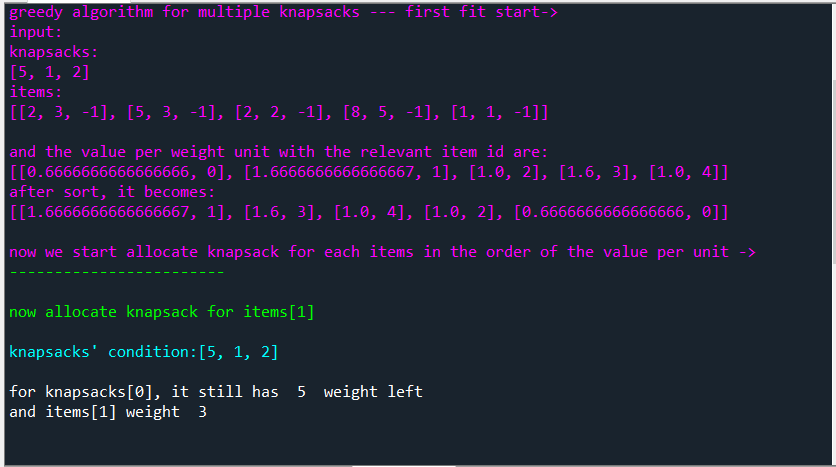
\includegraphics[scale=0.5]{process1}\\
That means we can observe the process of the program, that's the most direct way of correctness check.\\
for current example, the input of this algorithm will be:\\
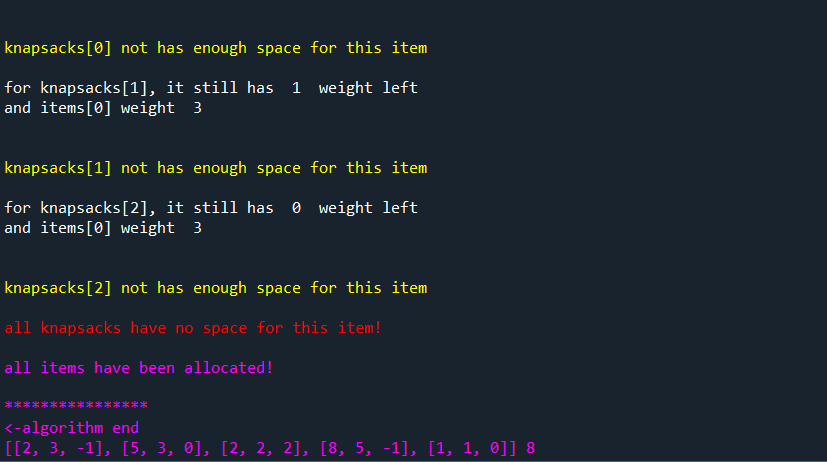
\includegraphics[scale=0.5]{result1}\\

\section{Neighbourhood search}
\subsection{mainly description for the algorithm}
Choose a suitable solution as the start solution, then find its best "neighbourhood" from all neighbourhood as the solution for the next iteration.When the best neighbourhood is even not better than the current one, then the algorithm end and output the current solution.
\subsection{implementation step}

\paragraph{step 1:} Choose a suitable solution as the start solution.
\paragraph{step 2:} while there are better neighbourhood existing, then choose the neighbourhood as the solution for next iteration. Redo this step continually.
\paragraph{step 3:} If the best neighbourhood is even not better than the current solution, the algorithm end and output the current solution.
\subsection{descriptions for some criteria}
\paragraph{neighbourhood definition:}On the base of the current solution, move one item to a certain knapsack. After removing a lowest value per unit item from this knapsack(if need), if there is enough space for this new item, then it is neighbourhood of the current solution.
\paragraph{termination criteria:}If the best neighbourhood is even not better than the current solution, the algorithm end and output the current solution.
\subsection{pseudo code}
\lstinputlisting[language=python]{pseudoCode2}
\subsection{code \& comment}
\lstinputlisting[language=python]{code2.m}
\subsection{correctness check \& test}
Like above saying that we can observe the process of the program.
we choose the output of the greedy algorithm as the start solution.\\
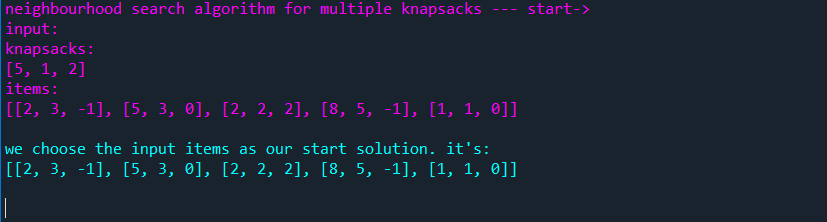
\includegraphics[scale=0.5]{process2}\\
and for each iteration, it will find neighbourhoods of current solution\\
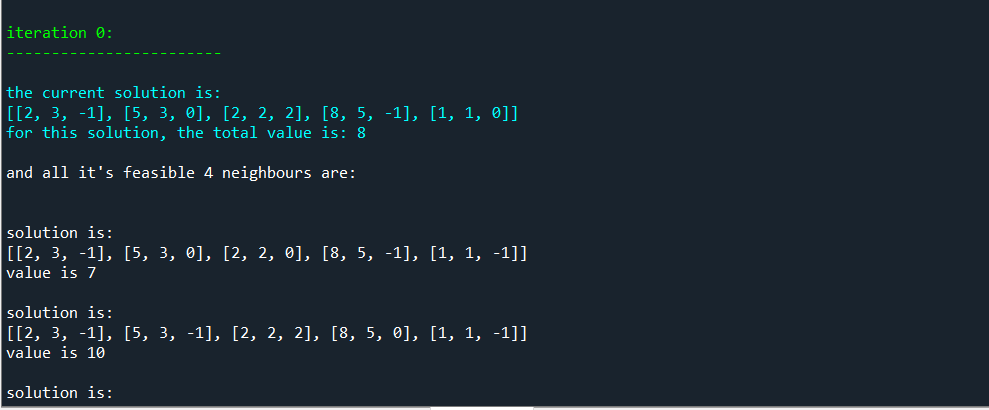
\includegraphics[scale=0.5]{process2_2}\\
and its output is\\
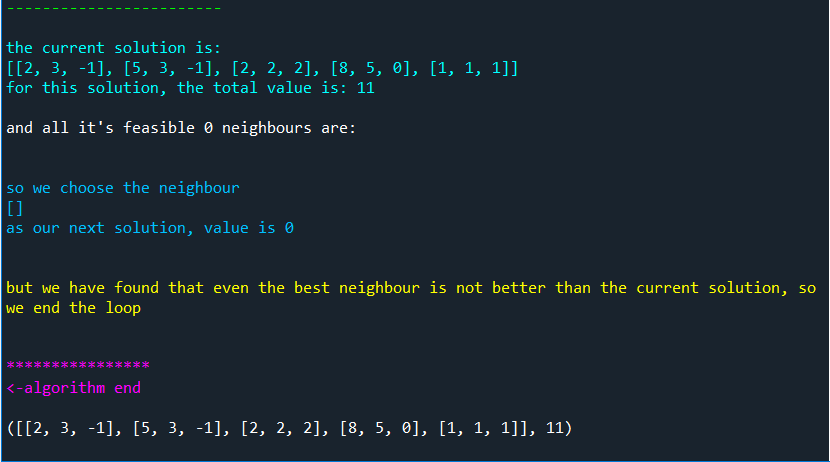
\includegraphics[scale=0.5]{result2}\\
\part{}
\section{Tabu-search}
\subsection{mainly description for the algorithm}
On the base of the neighbourhood search, we record the best solution when we search the neighbours.The difference is when we found that best neighbour is not better than the current one, we continue the algorithm until it reached the iteration times we provided. Also a tabu list will be used, we add the current solution into the list, and when the list is full, we replace the oldest solution in the list with the current one. all solutions in tabu list will be removed from the neighbours list.
\subsection{implementation step}

\paragraph{step 1:} Choose a suitable solution as the start solution.
\paragraph{step 2:} for each iteration, choose the best from those neighbourhoods are not inlcuded in the tabu list as the solution for next iteration. Redo this step continually.
\paragraph{step 3:} If the iteration times equals the given times, or there are no feasible alternative neighbours, end the algorithm.

\subsection{descriptions for some criteria}
\paragraph{neighbourhood definition:}On the base of the current solution, move one item to a certain knapsack. After removing a lowest value per unit item from this knapsack(if need), if there is enough space for this new item, then it is neighbourhood of the current solution.
\paragraph{tabu list length:}It was designed as a parameter that passed by user, that means we can choose to change the tabu list length to get different results.
\paragraph{termination criteria:}If the iteration times equals the given times, or there are no feasible alternative neighbours, end the algorithm.
\subsection{pseudo code}
\lstinputlisting[language=python]{pseudoCode3}
\subsection{code \& comment}
\lstinputlisting[language=python]{code3.m}
\subsection{correctness check \& test}
Like above saying that we can observe the process of the program.
we choose the output of the greedy algorithm as the start solution.\\
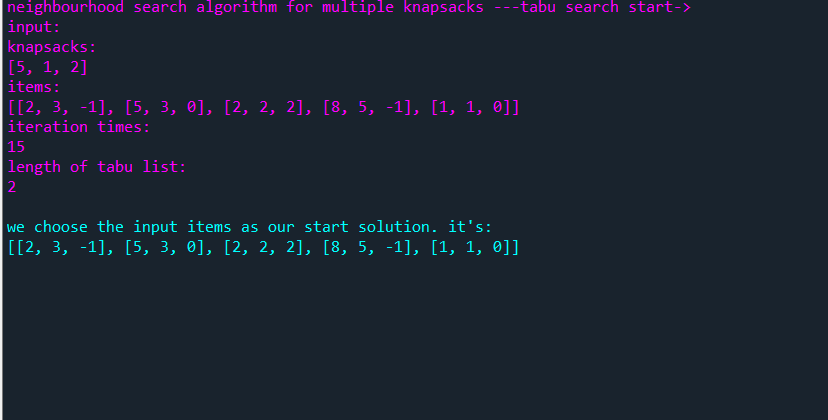
\includegraphics[scale=0.5]{process3}\\
in one iteration, the tabu list is\\
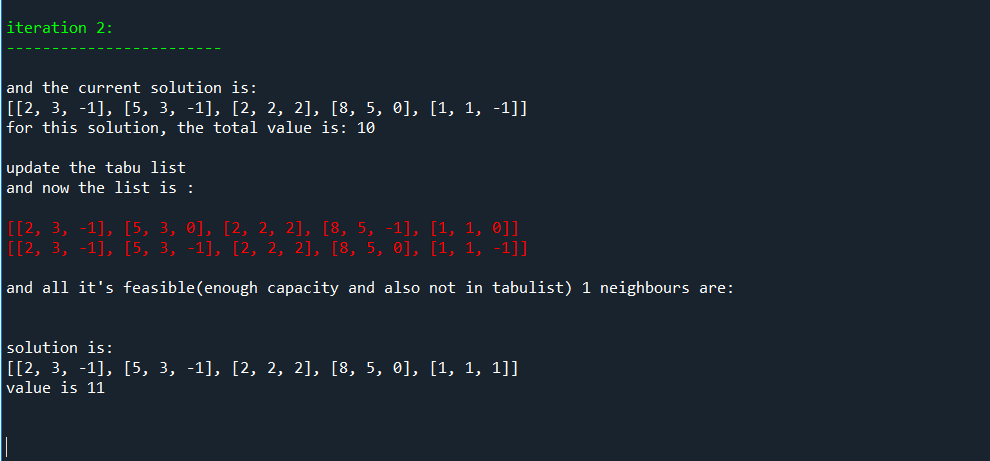
\includegraphics[scale=0.5]{process3_2}\\
and finally its output is\\
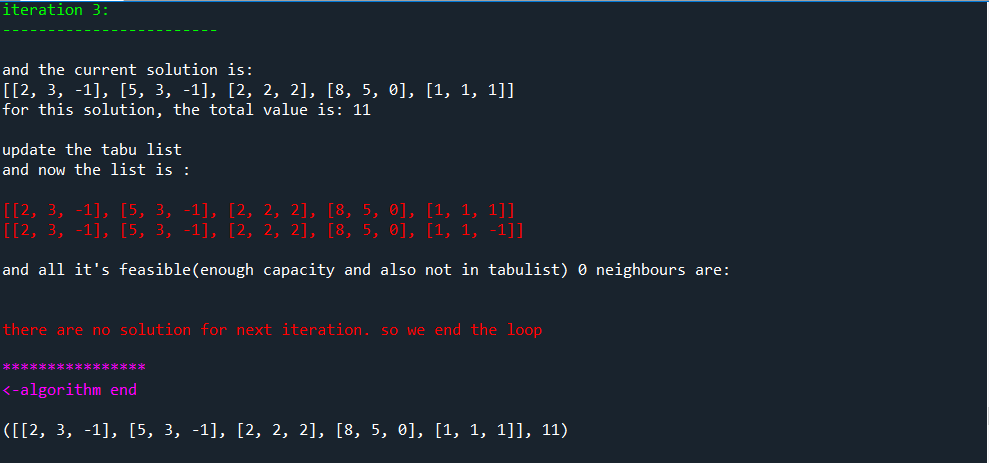
\includegraphics[scale=0.5]{result3}\\
\end{document}
